\documentclass[12pt]{report}

\usepackage{amsmath,braket,mathtools,bm}

\newcommand{\en}{\varepsilon}
\newcommand{\B}{\Gamma}
\newcommand{\s}{\sigma}
\newcommand{\sv}{\pmb{\sigma}}
\newcommand{\Nz}{\mathcal{N}}

\begin{document}

\subsection*{Edge mode in the TFI chain}
The spin-1/2 TFI chain of size $N$ with field in $x$:
%
\begin{equation*}
H = -J\sum_{n} \s^z_n \s^z_{n+1} + \B\sum_{n} \s^x_n,
\end{equation*}
%
has a normalized edge operator $\Psi = \Nz\s_1^z + \hat{O}(\B/J)$ which decays exponentially in $\B/J$ and almost commutes with $H$. This operator determines some matrix elements of $\s_1^z$. If we write $\s_1^z$ in the subspace of the two low-energy eigenstates $\ket{\pm}$, we have
%
\begin{equation}
\s_1^z =
\left(\begin{matrix}
0 & \Nz\\
\Nz & 0
\end{matrix}\right)
\end{equation}
%
where $\Nz^2 = 1 - (\B/J)^2$. When $\B \approx 0$, this operator relates well both low-lying states: $\s_1^z\ket{\pm} \approx \ket{\mp}$. However, this breaks down for $\B \sim J$, and to properly describe the (quasi)degeneracy of the ground state we need to use the full edge operator: $\Psi\ket{\pm} = \ket{\mp}$, and the operator is no longer localized at the edge after the phase transition at $\B = J$. Other edge operators with similar properties exist on models adiabatically related to TFI, for example on XY-Z and XZ-Z, and this also has consequences on $\s_1^z$. In particular, the second order expansion of $\Nz^2$ is
%
\begin{equation}
\Nz^2 \approx 1 - \sum_a \left( \frac{\theta_a}{J} \right)^2
\end{equation}
%
where we assume $J$ is the largest parameter of the model and where we sum over all other parameters $\theta_a$. All these operators can be built using an iterative method starting from $\s_1^z$ and successively calculating (guessing) higher order terms minimizing the commutator of the operator with $H$.

\subsection*{Edge mode in the staggered spin-1/2 Heisenberg chain}
We consider a staggered spin-1/2 Heisenberg chain (SHC) of size $N$ (even) with bonds $J_{F,AF}>0$:
%
\begin{equation*}
H = -J_F\sum_{n~odd} \sv_n \cdot \sv_{n+1} + J_{AF}\sum_{n~even} \sv_n \cdot \sv_{n+1}.
\end{equation*}
%
This Hamiltonian seems quite similar in form to TFI. For example, for $J_F = 0$, the two edge spins are completely decoupled and the ground state is degenerate, with the difference that the degeneracy is $4$. The appropriate basis for this subspace is $\{\ket{1,+},\ket{1,-},\ket{1,0},\ket{0,0}\}$, where
%
\begin{align*}
\ket{1,\pm} &= \ket{\pm}\otimes B \otimes\ket{\pm},\\
\ket{1,0} &= \ket{+}\otimes B\otimes\ket{-}+ \ket{-}\otimes B\otimes\ket{+},\\
\ket{0,0} &= \ket{+}\otimes B\otimes\ket{-}- \ket{-}\otimes B\otimes\ket{+},
\end{align*}
%
where $B$ is the bulk ground state. In this basis, $\s_1^z$ is
%
\begin{equation}
\s_1^z =
\left(\begin{matrix}
1 & 0 & 0 & 0\\
0 & -1 & 0 & 0\\
0 & 0 & 0 & 1\\
0 & 0 & 1 & 0
\end{matrix}\right).
\end{equation}
%
%
\begin{figure}
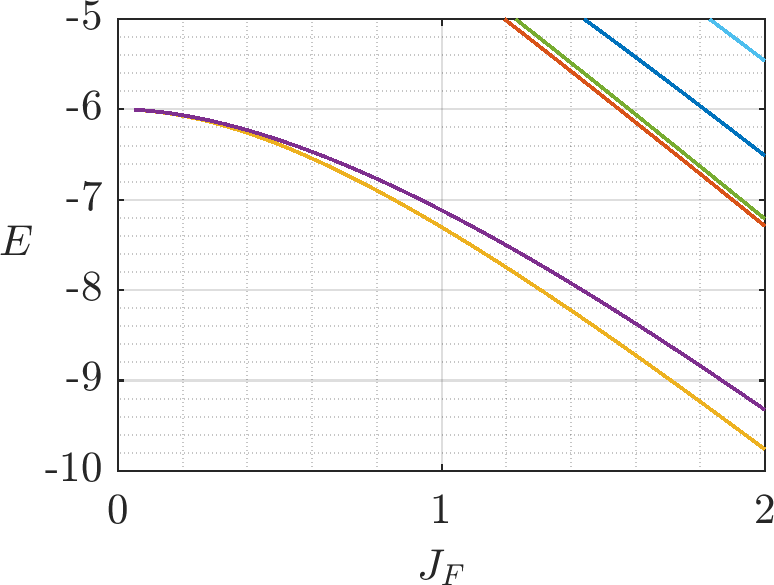
\includegraphics{Figures/Fig1b.png}
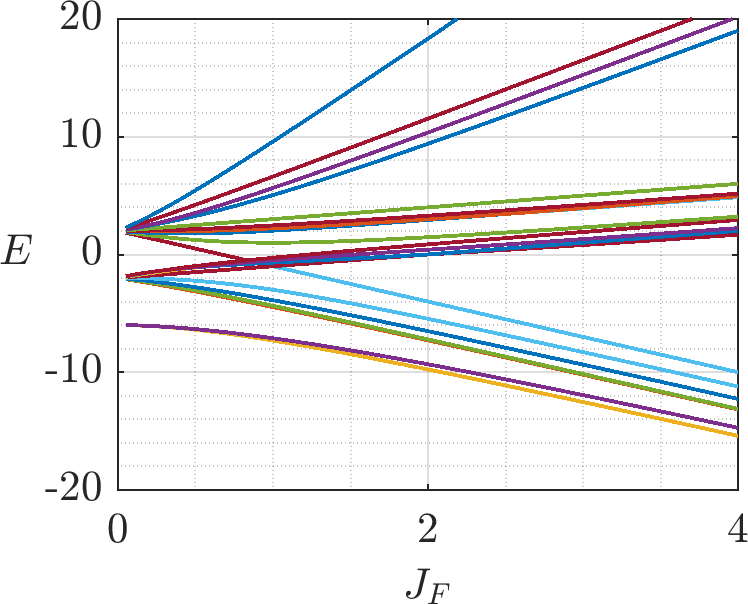
\includegraphics{Figures/Fig1a.png}
\caption{Spectrum of SHC for $J_{AF} = 1$, $N= 6$. Close-up on the left.}
\end{figure}
%
Then this operator relates the states $\ket{1,0}$ and $\ket{0,0}$. Another similarity with TFI is that when we turn on $J_F$ the energy difference between the singlet $\ket{0,0}$ and the triplet $\ket{1,m}$ remains small compared to the next excitation (Fig.~1). Due to these similarities with TFI, we wonder if it is possible to construct an operator $\Psi$ which is exponentially localized and is simply $\s_1^z$ in zero order in $J_F$. I believe this is not possible. By comparison with TFI, we would guess the base of the exponentiation to be $J_F/J_{AF}$. However, this might be a bit naive, since this would give a special importance to the situation $J_F=J_{AF}$, but while in TFI there is a phase transition at the equivalent point, in SHC there is no phase transition for $J_F>0$, so even considering a more general base $\alpha J_F/J_{AF}$ does not make sense. Also, the analytic method fails to provide us with such an operator, mainly because the constraint of minimizing the commutator $[\Psi,H]$ has strong  consequences on the whole spectrum, in particular a small commutator implies a quasi-degeneracy of all energy levels, and while the low lying states obey this, the same is not observed in the rest of the spectrum. Let us look at the elements of $\s_1^z$ as a function of $J_F$. Fixing $J_{AF} = 1$, we plot in Fig.~2 both non-zero degrees of freedom of $\s_1^z$, which for non-zero $J_F$ is of the form
%
\begin{equation}
\s_1^z =
\left(\begin{matrix}
A & 0 & 0 & 0\\
0 & -A & 0 & 0\\
0 & 0 & 0 & B\\
0 & 0 & B & 0
\end{matrix}\right).
\end{equation}
%
%
\begin{figure}
\centering
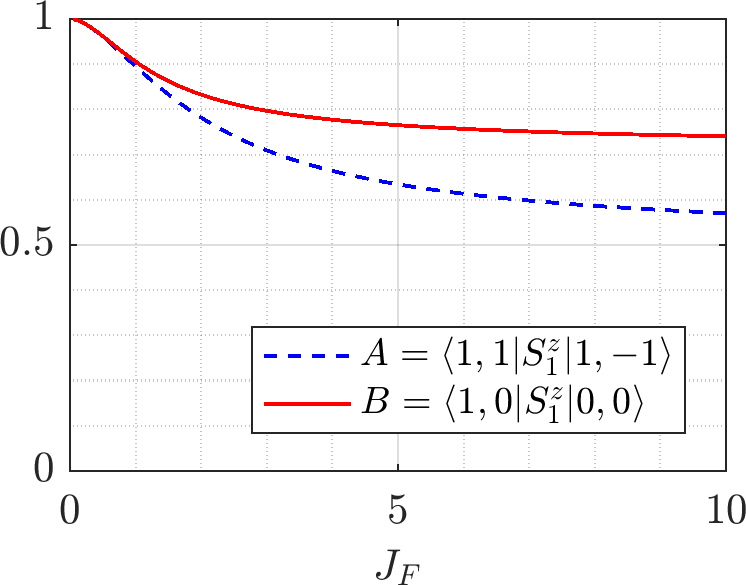
\includegraphics{Figures/Fig2.png}
\caption{Matrix elements of $S_1^z$ with $J_{AF} = 1$, $N= 8$.}
\end{figure}
%
While the matrix elements of $\s_1^z$ on TFI reflect the existence of a phase transition, here we don't see any change in behaviour, as expected, but also the elements do not seem to go to zero even for infinite $J_F$. I would say this means the singlet and the triplet are still related by the edge spin $1/2$ and we don't need a decaying operator to describe this.

\subsubsection*{Question}
Both $A$ and $B$ approach some value ($\sim0.5$ and $\sim0.7$ respectively) in the limit $J_F \rightarrow \infty$. How could we obtain these values exactly? We should be able to use somehow the exact solution of $J_{AF}=0$.

\end{document}
